%%%%%%%%%%%%%%%%%%%%%%%%%%%%%%%%%%%%%%%%%%%%%%%%%%%%%%%%%%%%%%%%%%%%%%%%%%%%%%%%
%2345678901234567890123456789012345678901234567890123456789012345678901234567890
%        1         2         3         4         5         6         7         8

%\documentclass[letterpaper, 10 pt, conference]{ieeeconf}  % Comment this line out
                                                          % if you need a4paper
\documentclass[a4paper, 10pt, conference]{ieeeconf}      % Use this line for a4
                                                          % paper

\IEEEoverridecommandlockouts                              % This command is only
                                                          % needed if you want to
                                                          % use the \thanks command
\overrideIEEEmargins
% See the \addtolength command later in the file to balance the column lengths
% on the last page of the document



% The following packages can be found on http:\\www.ctan.org
%\usepackage{graphics} % for pdf, bitmapped graphics files
\usepackage{epsfig} % for postscript graphics files
%\usepackage{mathptmx} % assumes new font selection scheme installed
%\usepackage{times} % assumes new font selection scheme installed
%\usepackage{amsmath} % assumes amsmath package installed
%\usepackage{amssymb}  % assumes amsmath package installed

\title{\LARGE \bf
Autonomous Offensive Passing Systems for Robot Soccer
}

%\author{ \parbox{3 in}{\centering Huibert Kwakernaak*
%         \thanks{*Use the $\backslash$thanks command to put information here}\\
%         Faculty of Electrical Engineering, Mathematics and Computer Science\\
%         University of Twente\\
%         7500 AE Enschede, The Netherlands\\
%         {\tt\small h.kwakernaak@autsubmit.com}}
%         \hspace*{ 0.5 in}
%         \parbox{3 in}{ \centering Pradeep Misra**
%         \thanks{**The footnote marks may be inserted manually}\\
%        Department of Electrical Engineering \\
%         Wright State University\\
%         Dayton, OH 45435, USA\\
%         {\tt\small pmisra@cs.wright.edu}}
%}

\author{Alex Cunningham and Philip Rogers% <-this % stops a space
\thanks{This work was not supported by any organization}% <-this % stops a space
% \thanks{H. Kwakernaak is with Faculty of Electrical Engineering, Mathematics and Computer Science,
%         University of Twente, 7500 AE Enschede, The Netherlands
%         {\tt\small h.kwakernaak@autsubmit.com}}%
% \thanks{P. Misra is with the Department of Electrical Engineering, Wright State University,
%         Dayton, OH 45435, USA
%         {\tt\small pmisra@cs.wright.edu}}%
}


\begin{document}



\maketitle
\thispagestyle{empty}
\pagestyle{empty}


%%%%%%%%%%%%%%%%%%%%%%%%%%%%%%%%%%%%%%%%%%%%%%%%%%%%%%%%%%%%%%%%%%%%%%%%%%%%%%%%
\begin{abstract}

This project adds new passing capabilities to the GT Robojackets RoboCup Small Size League (SSL) robot team. The existing system supports moving, shooting, and can play the rules of soccer, but does not currently handle multirobot activity, such as passing, in a reliable manner. We extend the current system to implement a robust offensive passing system where the robots will acquire ball control and then make a coordinated series of passes until it can shoot on goal. We demonstrate a multi-stage planner that creates initial plans with an analytical planner and then performs nonlinear constrained optimization over the positions of robots to create an improved plan that mixed low-level controllers can execute.  

\end{abstract}


%%%%%%%%%%%%%%%%%%%%%%%%%%%%%%%%%%%%%%%%%%%%%%%%%%%%%%%%%%%%%%%%%%%%%%%%%%%%%%%%
\section{INTRODUCTION}
One of the larger robotics competitions in the world is the RoboCup competition, which seeks to build a robot soccer team that can beat a World Cup human team by the year 2050.  The subdivision in this project is the RoboCup Small Size League (SSL), in which a team plays 5-on-5 autonomous soccer.  What is notable about this league, is that due to the small size of the robots and omnidirectional drivetrain, the robots are extremely fast and agile, to a degree where humans are not capable of manually driving the robots nearly as well as autonomous control.  Due to this speed, SSL games provide an interesting domain for planning problems, as they are capable of playing a rather sophisticated game of soccer.  

The robot platform includes a team of robots controlled remotely via a centralized computer system, with an overhead vision system to determine the global position of the robots.  The centralization of the processing avoids many of the difficulties of using a true decentralized system, and as such more sophisticated gameplay occurs.  Our research builds on the existing system developed as a part of the Georgia Tech Robojackets RoboCup SSL team, currently ranked 2nd in the US, which includes a full fleet of robots and a simulator environment, in addition to the full robot control system.  

This project is an interesting planning challenge because of the speed of the robots and play that occurs in these games. Unlike the humanoid or four-legged-leagues, the Small Size League (SSL) robots are extremely fast in both motion and shooting, which makes the soccer games fast-paced, and reliant on effectively solving a number of sophisticated planning challenges simultaneously. To implement a basic passing system, the robots need to be able to move and plan in their space effectively, which is a non-trivial challenge because the robots have high enough acceleration to flip themselves over if they stop too quickly. Once a robot has a ball, the other robots need to position themselves to both receive an incoming pass and make another pass. While the number of robots is relatively small, such that a simple graph search can produce a series of passes to shoot on goal, handling the dynamic conditions of a high-speed game forces the planner to be more sophisticated. Because this is a soccer game, the primary 'obstacles' on the field are not just static or even dynamic obstacles, they are adversarial robots that will attempt to disrupt any plan execution that occurs. An effective planner in for these challenges must simultaneously manage basic motion planning for the robots, model passing sufficiently well to pass between the robots, find and replan optimal positions for robots. The additional constraint on the system is the uncertainty of the measurement, as there is noise in the robot position measurements, and especially the ball, which will disappear off of the global vision system if it moves too fast - a scenario that occurs almost every time a shot is made. 

\section{Related Work}

% this is put here to force it onto page 2 (at the end of related work)
% this is referenced in our methods section though.
\begin{figure*}[ht!]
\begin{center}
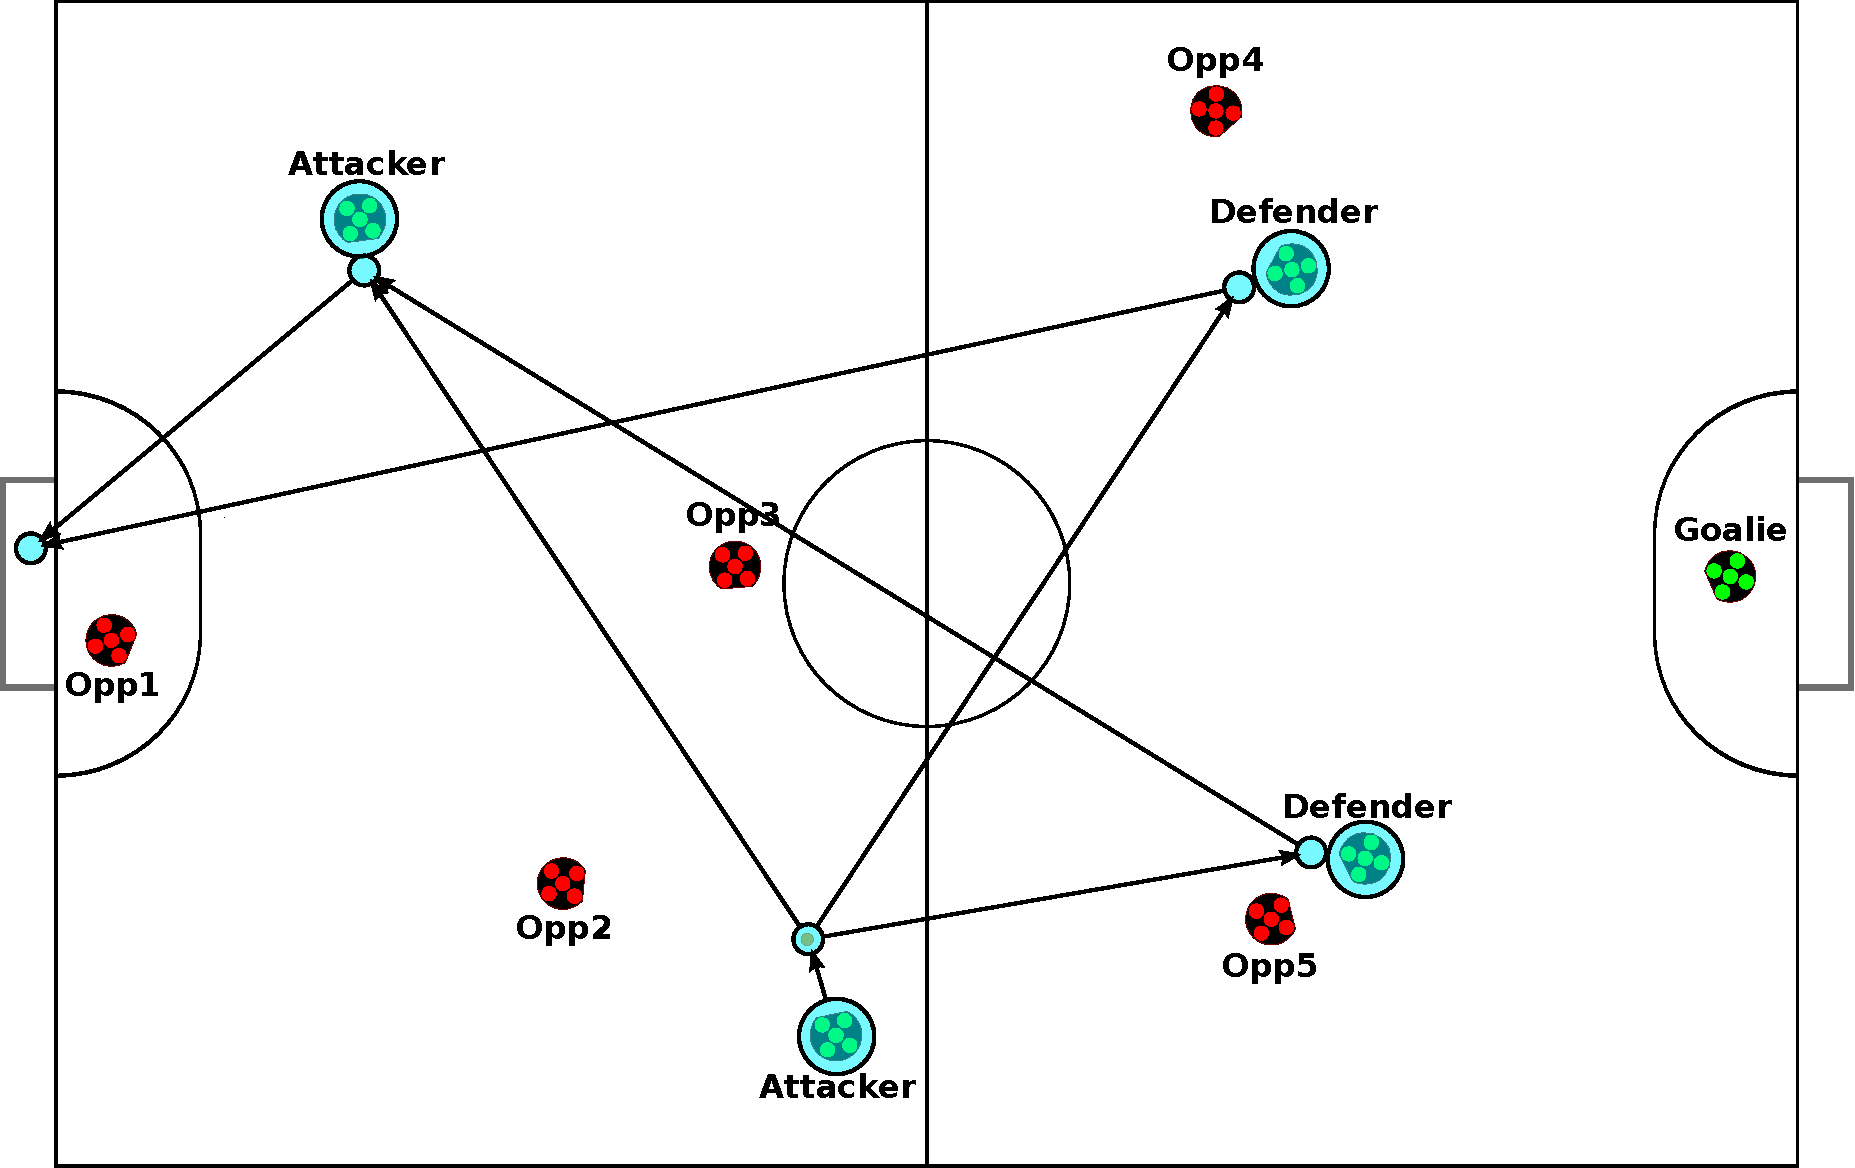
\includegraphics[totalheight=1.0in]{plan2_resized}
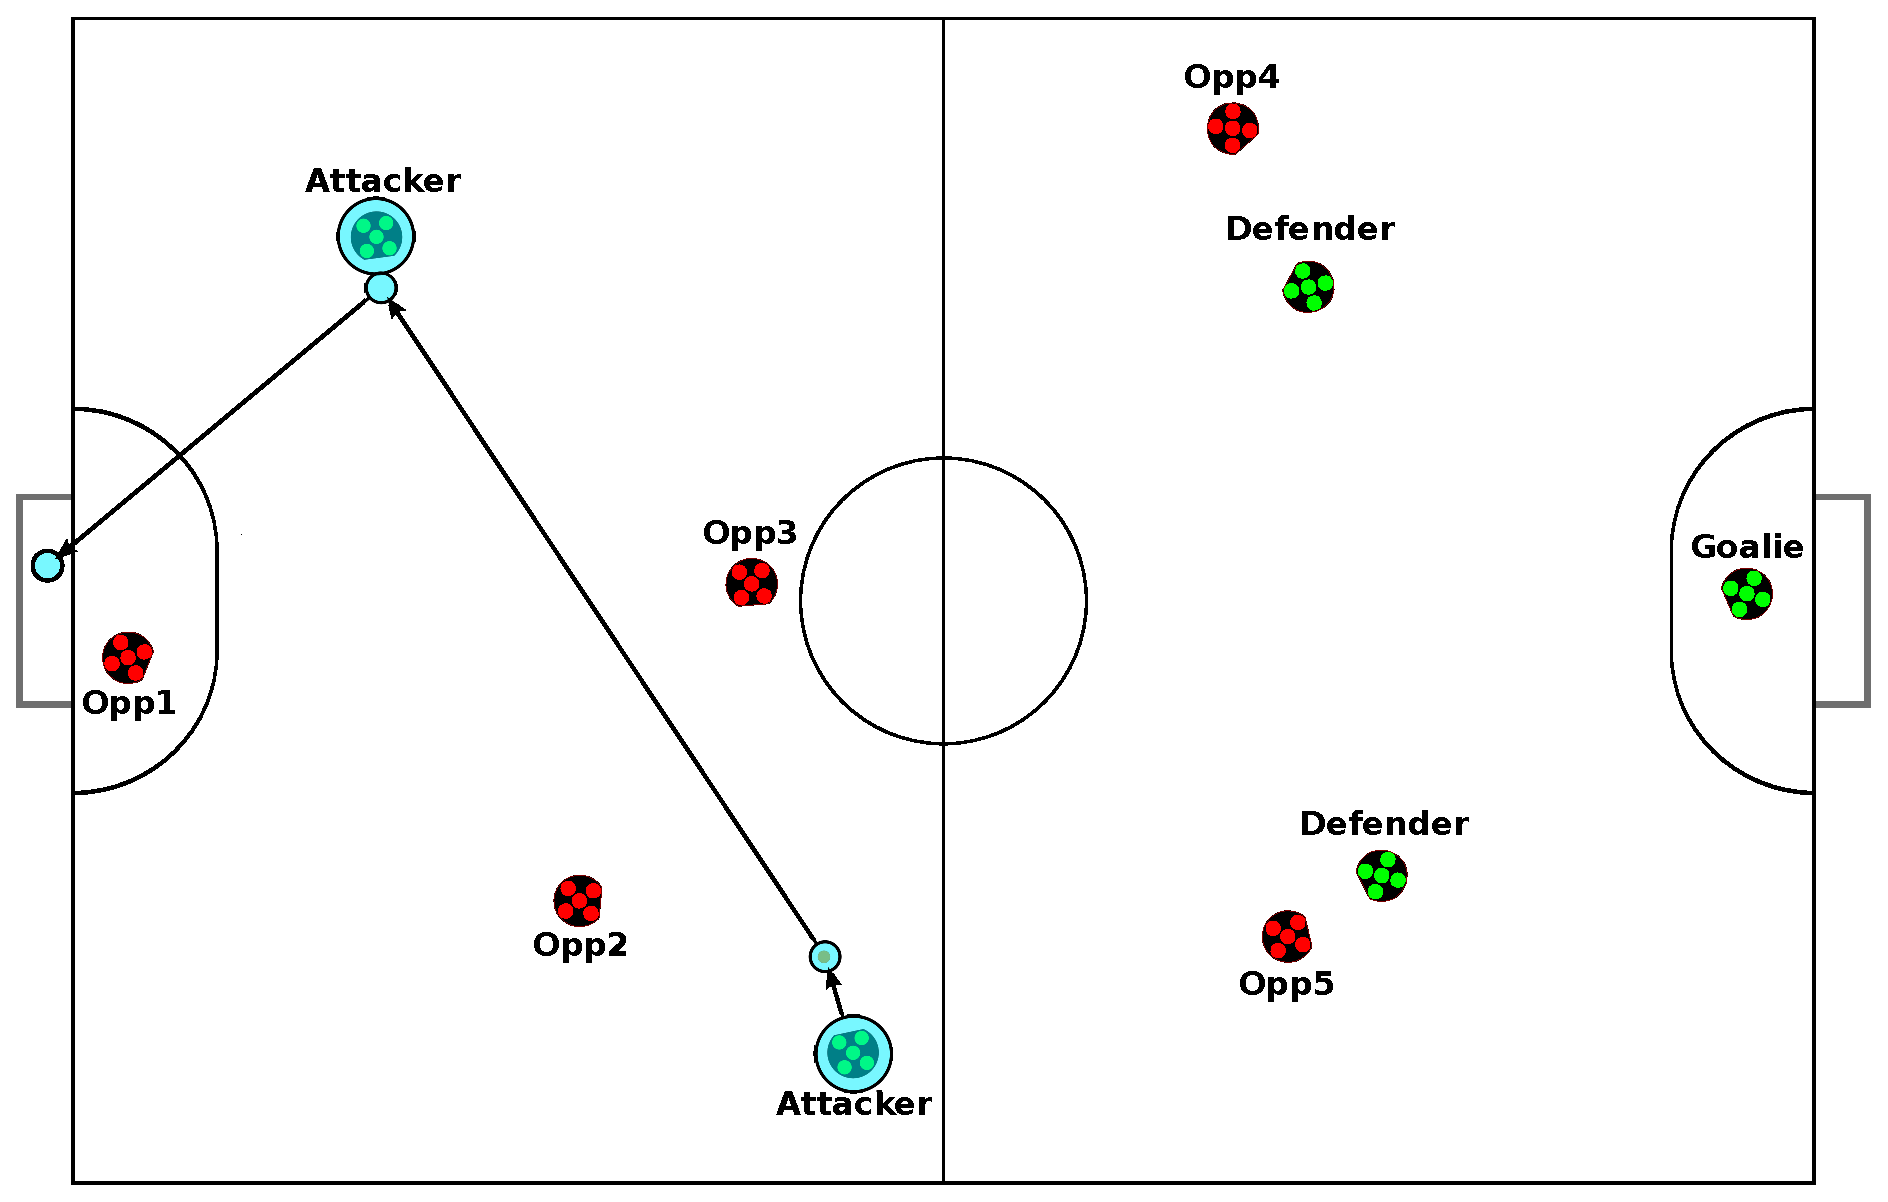
\includegraphics[totalheight=1.0in]{plan3_resized}
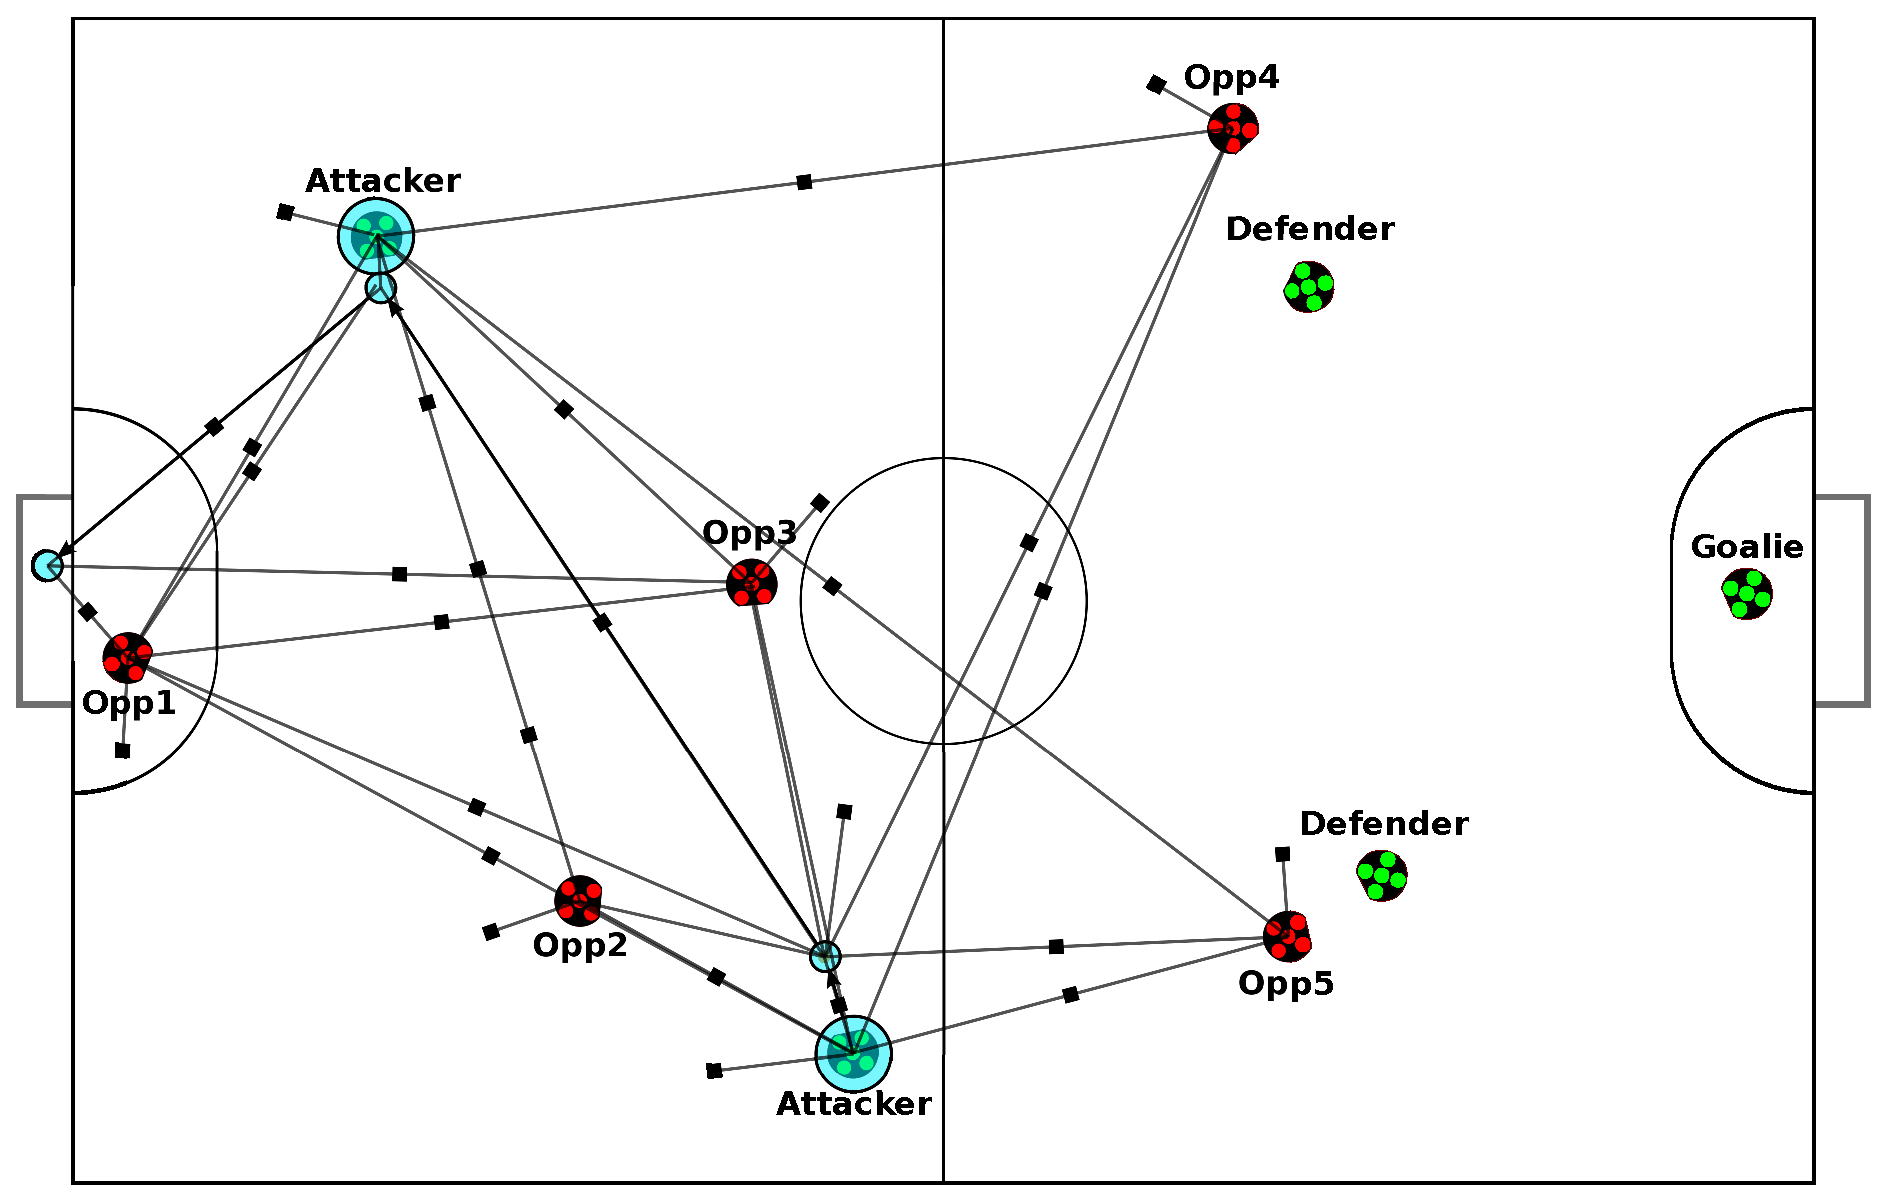
\includegraphics[totalheight=1.0in]{plan5_resized}
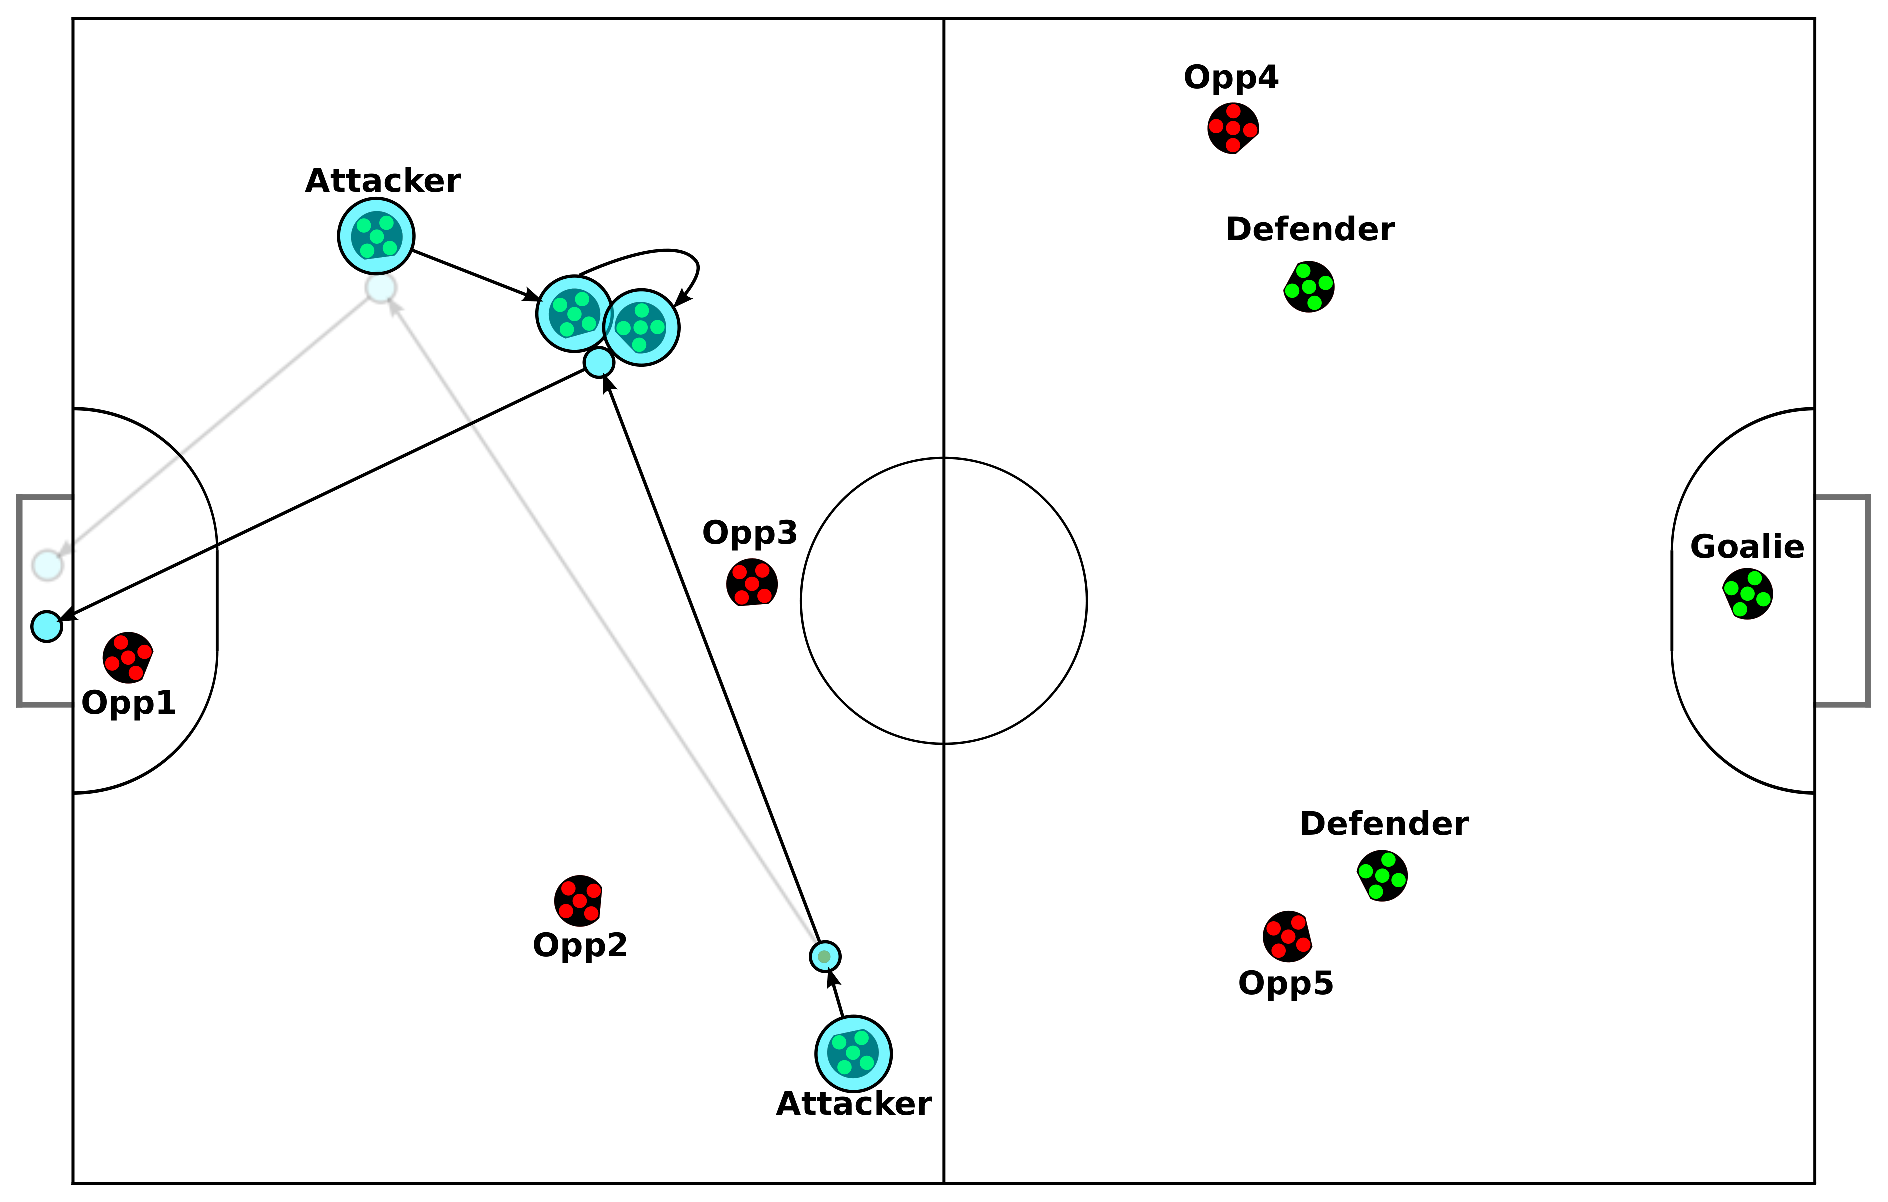
\includegraphics[totalheight=1.0in]{plan4_resized}
\end{center}
\caption{Methods used: Left-to-right: (1.) Analytic planner result (2.) Plan evaluation and selection of feasible subset. (3.) Optimization of feasible subset of plans. (4.) Optimized result which is executed.}
\end{figure*}

The Skills, Tactics and Plays (STP) framework is the primary technique used by top Robocup teams \cite{cmdragonsETD, skubaETD}. STP is a hierarchical approach where 
dfdsfds test \cite{browning2005stp,bruce2003multi,zickler2008playing,bruce2003real}
"STP: Skills, tactics and plays for multi-robot control in adversarial environments" Brett Browning, James Bruce, Michael Bowling, and Manuela Veloso, Journal of System and Control Engineering (2005). This paper is the primary technique used by top RoboCup teams for planning both locally (kicking) and globally (passing) in the soccer domain. We have a rudimentary implementation of the STP framework currently, but it does not support global planning at the level required for competitive play. One of the main goals of our project is to extend our existing implementation, as the STP paper describes, to support passing and generally improved global teamplay.

"Multi-robot team response to a multi-robot opponent team" James Bruce, Michael Bowling, Brett Browning, and Manuela Veloso, ICRA '03. This paper describes the CMDragons implementation of Skills, Tactics, and Plays (STP) framework, and how they use it to achieve teamwork plays such as passing. It presents an example of their playbook, which is also published in full online, and can be used as a starting point for our passing implementation. The CMDragons team uses extensive passing, including "One-touch" kicking and chip-kick passing.

"Real-Time Randomized Path Planning for Robot Navigation" James Bruce, Manuela Veloso, IROS '02. This paper describes a modification the RRT algorithm called "execution extended RRT" (ERRT) that improves the efficiency of the RRT algorithm by weighting the search-space and improving replanning. Both of these topics are directly applicable to the RoboCup domain, where adversarial players affect the search space, and replanning is constantly occurring. By using ERRTs, our goal is to be able to create more efficient plans at the local planning level, which will lead to improved global plans.

"Map-based Multiple Model Tracking of a Moving Object" Cody Kwok, Dieter Fox, Proceedings of RoboCup Symposium, 2004. Due to the camera position, it is common to lose track of the soccer ball when multiple robots are occluding the camera's view. This paper presents a Rao-Blackwellized Particle Filter (RBPF) for tracking of the ball. It uses a technique of using particle filters for the non-linear portion of the tracking, and an Extended Kalman Filter (EKF) for the linear portions. Examples of the non-linear ball dynamics are during kicking, bouncing, etc. We hope this will improve overall planning, and is a requirement for passing.

\section{METHODS}
In order to perform robust, efficient passing, we have decided on a particular structure for the offense play. The basic concept is that if there is a shot available or a sequence of passes to a shot (henceforth known as a "shooting solution"), then the system will construct the sequence of paths for robots and kicks, run a nonlinear optimization technique to improve the path and ensure viability, and then execute it.

This plan came out of two particular observations:

\begin{itemize}
 \item This bypasses the existing RRT-based planner, which is too unpredictable in timing for highly coordinated actions. We have no particularly good way of telling when a robot will reach a location when using RRTs.
 \item Because of the particular scenario of robot soccer, we know there are a small number of obstacles on the field, and there are only a small number of possible paths between them. With an optimization algorithm, we can take a simple path and improve it to make it faster.
\end{itemize}

The resulting system structure for the offensive passing algorithm has the following structure:
\begin{enumerate}
 \item \textit{Analytic Planner} Given the positions of all the robots and the ball, it is possible to determine if there is a shot solution available with a simple weighted graph search. This can be a simple heuristic for shot viability, or a more sophisticated system as necessary.
 \item \textit{Plan Evaluation} We take a set of plans and sort by quality on a number of metrics, so that a good initial estimate can be created.
 \item \textit{Optimization} With an initial estimate of a plan, the optimization engine will be able to create a graphical model of the plan and optimize for an optimal sequence of actions. The particular optimization engine is a nonlinear constrained optimization algorithm primarily designed for Simultaneous Localization and Mapping, but we will exploit the duality between this planning problem (create an optimal path from constraints) and SLAM (recover a previously traveled path given measurements).
 \item \textit{Execution} Given a viable plan a variety of motion planning and behavioral approaches can be used to to execute the actions that have been parameterized by plan generation and optimized.  
\end{enumerate}

The optimization algorithm comes from the gtsam library\cite{Dellaert05rss} developed in the RIM center with Frank Dellaert, and is derived from Sequential Quadratic Programming. This algorithm is robust to both nonlinear systems and constraints, and has been reformulated to work in a graphical model environment, which allows for an intuitive construction of stochastic switched hybrid systems.

\textit{TODO: Describe the actual analytic planner system}

\textit{TODO: Describe the optimizer in mathematical detail and formulation of the constraints and factors}

\section{EXPERIMENTS}
We tested the system using the simulated environment with the GT RoboCup software, which allows for an identical interface between the simulated environment and the real robots.  

\begin{figure}[ht!]
\begin{center}
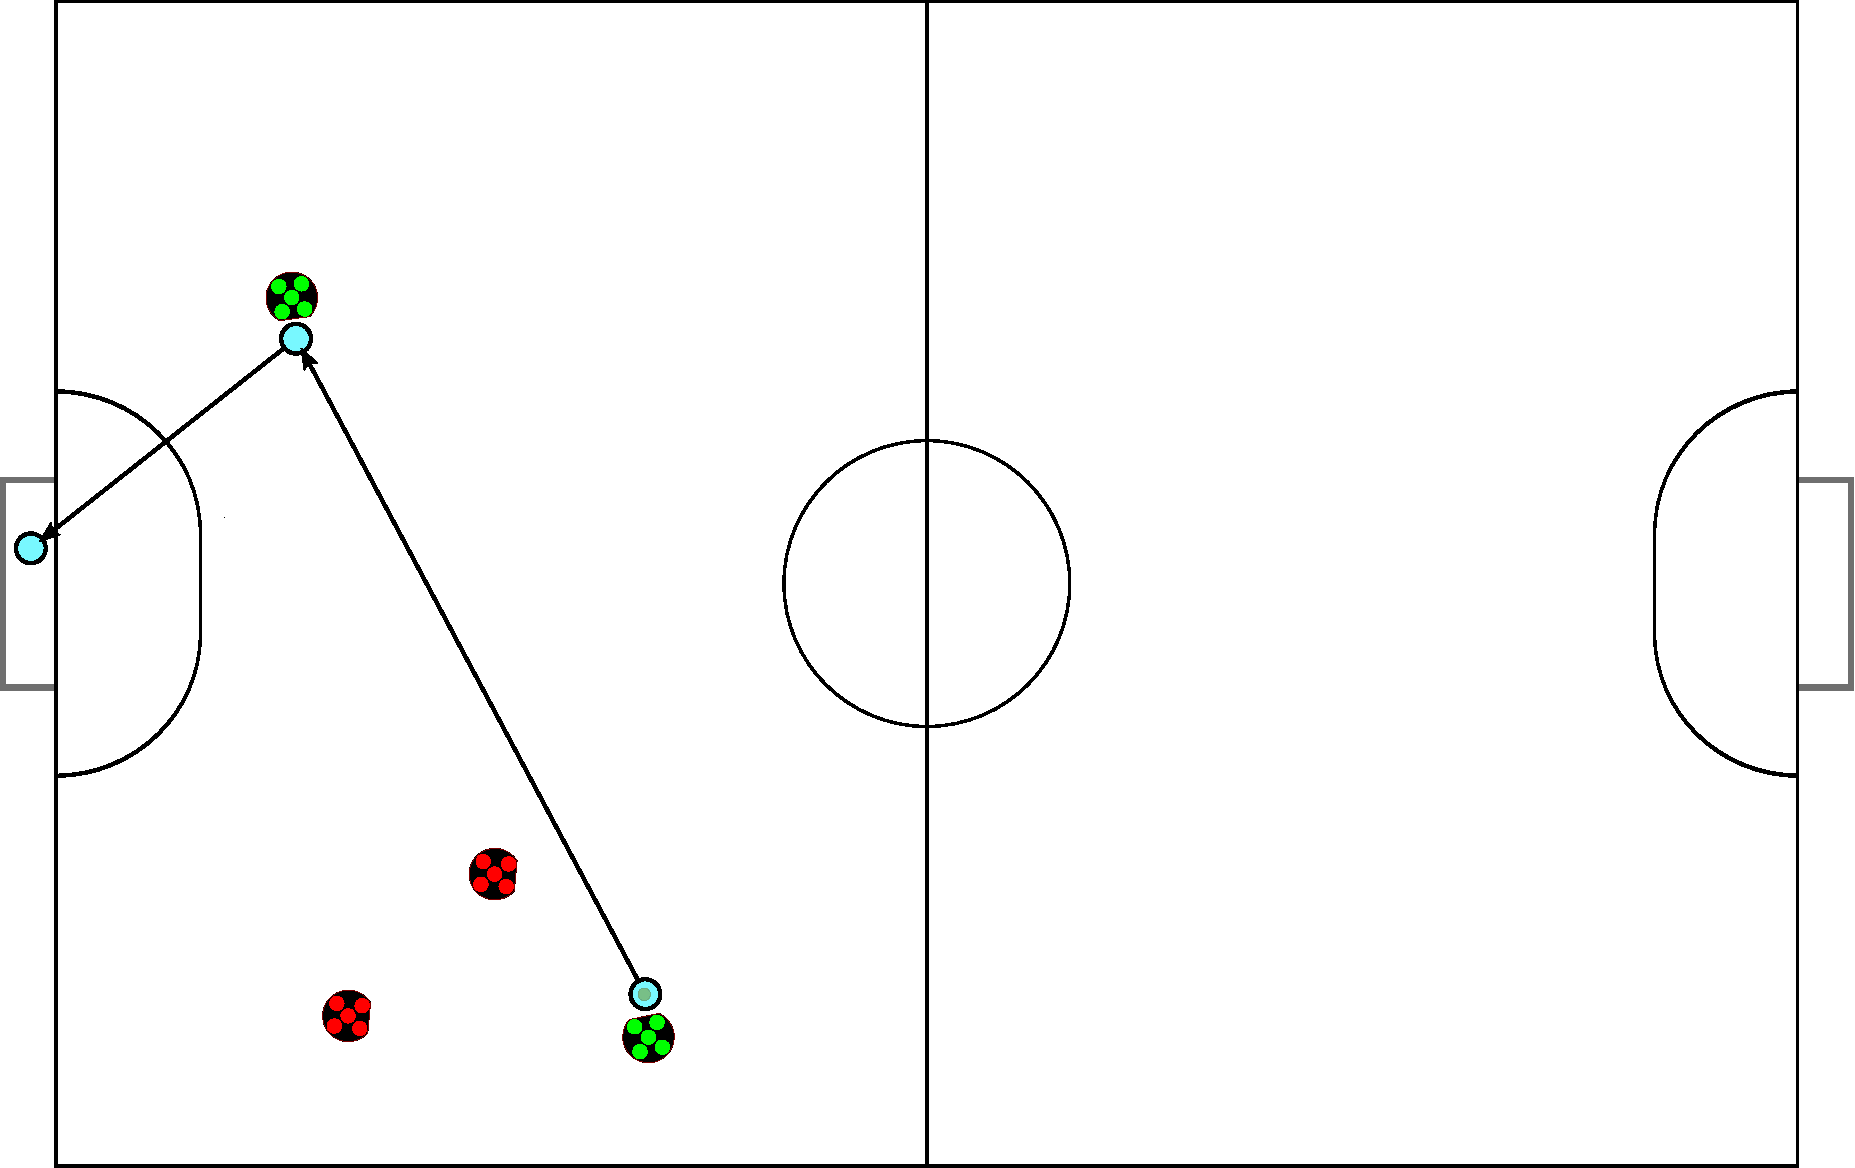
\includegraphics[totalheight=1.0in]{nonoptimized_plan}
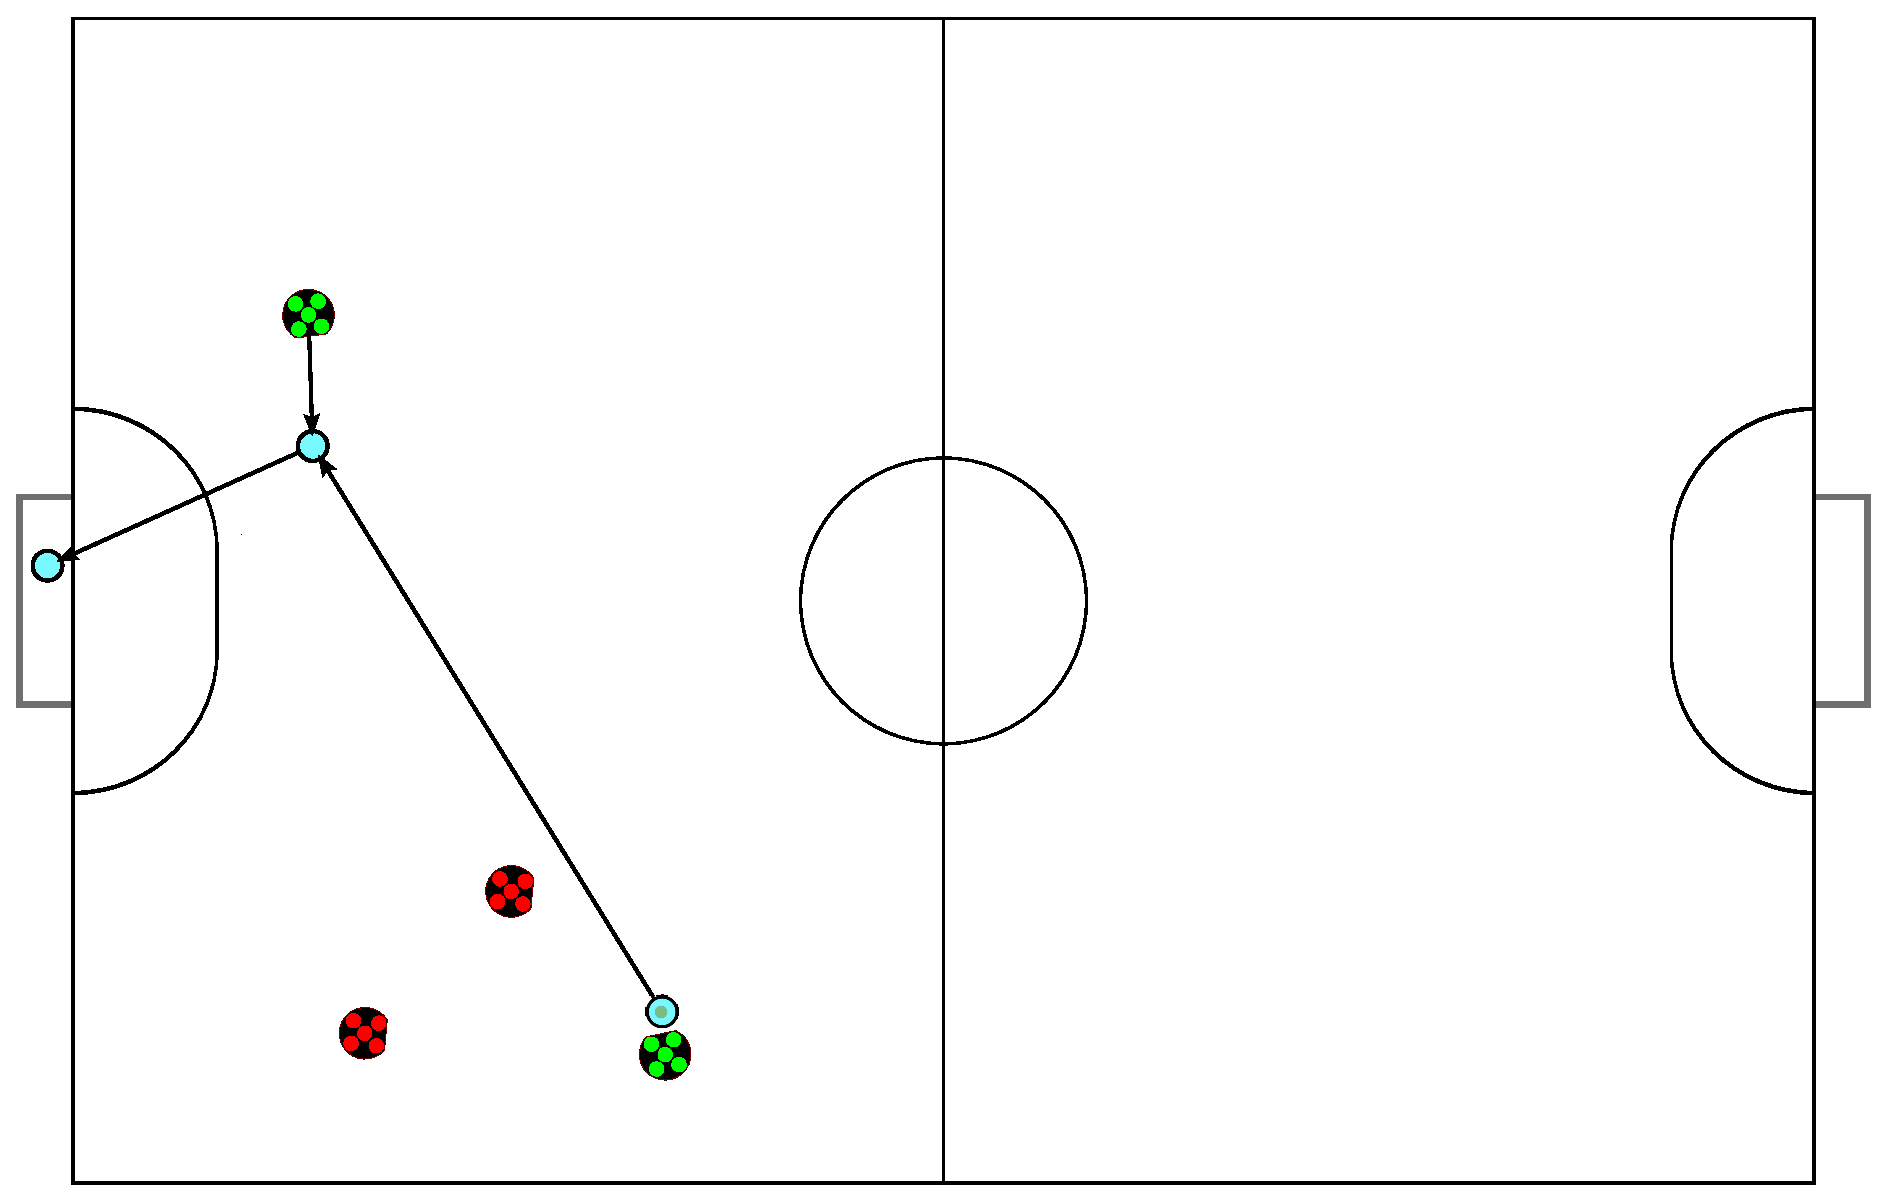
\includegraphics[totalheight=1.0in]{optimized_plan}
\end{center}
\caption{Left: naive pass, execution took 5 seconds. Right: optimized path, execution took 4 seconds.}
\end{figure}

\textit{TODO: insert some results here}

\section{ANALYSIS}
The results of the system, in a somewhat simplified form, indicate potential for this process.

\section{DISCUSSION}
We learned a number of lessons from the development of this system, and there is a great deal that can be improved, but the combination of an analytic planner and an optimization engine appear to be an effective means of generating passing plans.  The optimizer has a great deal of flexibility, and even in a smaller example system, we have the flexibility to make the system very robust.  Further work could improve the system by integrating a motion model into the factor graph itself, and then bypassing the underlying RRT-based planner to make plans more predictable. 
\begin{itemize}
\item The multi-stage planner allows evaluation of plans we would not have been able to find otherwise
\item While the current optimization approach uses a simpler cost function, the system is very scalable
\item We need to improve the interactions between the low-level control and the planner outputs
\end{itemize}


%%%%%%%%%%%%%%%%%%%%%%%%%%%%%%%%%%%%%%%%%%%%%%%%%%%%%%%%%%%%%%%%%%%%%%%%%%%%%%%%

\section{ACKNOWLEDGMENTS}

The authors would like to thank the GT RoboCup SSL team for developing the system used for this project, and in particular Ben Johnson and the rest of the software team for managing many of the background details of keeping the entire robot control system functional. 


\bibliographystyle{unsrt}
\bibliography{RIPFinal}
% \begin{thebibliography}{99}
% 
% \bibitem{c1}
% J.G.F. Francis, The QR Transformation I, {\it Comput. J.}, vol. 4, 1961, pp 265-271.
% 
% \bibitem{c2}
% H. Kwakernaak and R. Sivan, {\it Modern Signals and Systems}, Prentice Hall, Englewood Cliffs, NJ; 1991.
% 
% \bibitem{c3}
% D. Boley and R. Maier, "A Parallel QR Algorithm for the Non-Symmetric Eigenvalue Algorithm", {\it in Third SIAM Conference on Applied Linear Algebra}, Madison, WI, 1988, pp. A20.
% 
% \end{thebibliography}

\end{document}
